\documentclass[11pt]{article}
\usepackage[a4paper,margin=1in]{geometry}
\usepackage{amsmath,amssymb}
\usepackage{microtype}
\usepackage[hidelinks]{hyperref}
\usepackage{tikz}
\usepackage{amsthm}
\usepackage{graphicx}
\theoremstyle{plain}
\newtheorem{lemma}{Lemma}[section]


\theoremstyle{definition}
\newtheorem{definition}{Definition}[section]

\theoremstyle{remark}
\newtheorem{remark}{Remark}[section]


\usetikzlibrary{arrows.meta,decorations.pathreplacing,positioning}
\usepackage{enumitem}
\title{\large\bfseries CEGS Demonstration\\[4pt]
\large Emergent Structure via a Wavefront R\textsuperscript{3} $\rightarrow$ \(\mathbb{C}\) Mapping}
\author{Norman De Leeuw}
\date{}

\begin{document}
\maketitle

\noindent\textbf{Purpose.} Provide a short, physically oriented demonstration of how the Calculus of Element Generated Sets (CEGS) maps three dimensional geometric wavefronts into structurally complete complex-valued functions on a plane. This demonstration highlights two mechanisms: (1) a reversible encoding of $\mathbb{R}^3$ geometry as complex functions, and (2) orthogonality lifting — the temporary deferral of Euclidean relational comparison that allows symbolic constraint closure to produce emergent structures.

\vspace{6pt}
\noindent\textbf{Key idea (intuitive).}  
Imagine an evolving wavefront (e.g., an expanding spherical wave emitted by a localized source). Instead of projecting this wavefront onto a screen as a static pointwise image, CEGS associates each point \(p\in\mathbb{R}^3\) with a \emph{local complex function} \(F_p: \mathbb{C}\to\mathbb{C}\). Each screen location \(z\in\mathbb{C}\) becomes a function carrier rather than a single amplitude value. Under this association the entire 3D wavefront is encoded as a coherent family of complex functions; constraints (physical boundary conditions, symmetry, propagation rules) then act as symbolic operators that collapse, reorganize, or reveal emergent stable structures in the function family.
\begin{figure}[h!]
\centering
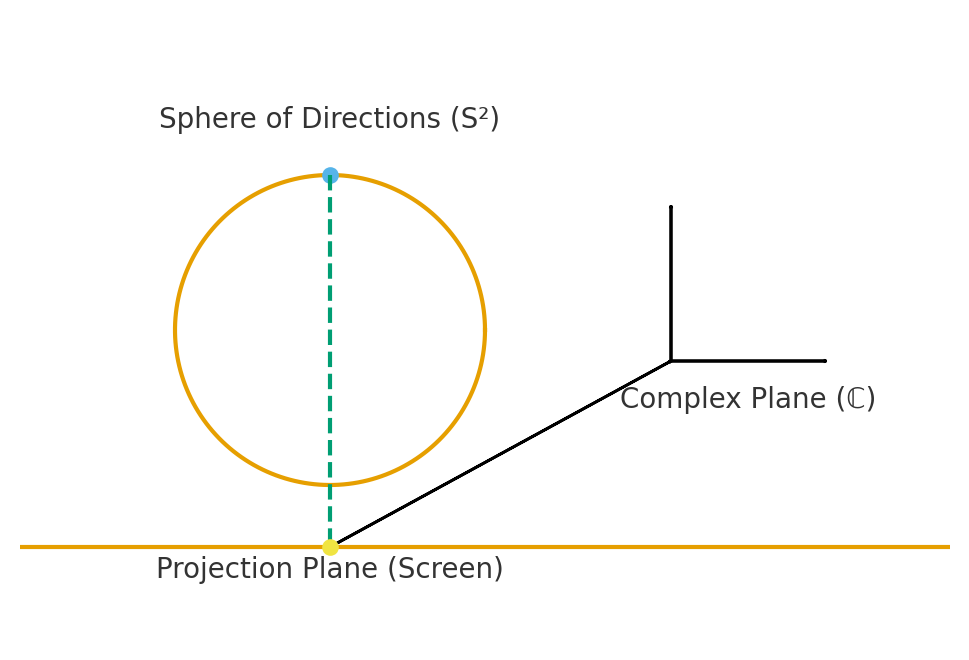
\includegraphics[width=0.85\textwidth]{C2_Projection.png}
\caption{Illustrative example of the $\mathbb{R}^2 \rightarrow \mathbb{C}^1$ mapping. 
Each point in $\mathbb{R}^2$ corresponds to a complex-valued function, forming 
a structural analogy to the symbolic encoding used later in the $\mathbb{R}^3 \rightarrow \mathbb{C}$ wavefront model.}
\label{fig:R2C1mapping}
\end{figure}

\vspace{6pt}
\noindent\textbf{Orthogonality lifting (precise meaning).}  
CEGS does \emph{not} alter or remove the internal orthogonality between the real and
imaginary axes in $\mathbb{C}$ (i.e., $1 \perp i$ remains intact). What is lifted is the
\textbf{external Euclidean comparability} between complex-valued symbolic objects.
That is, two generated complex functions $F_p$ and $F_q$ are \emph{not} interpreted as
points in a metric plane to be compared by Euclidean distance; instead, they are
symbolic objects whose relationships are determined only after constraints are
applied. This deferment of metric comparison is what enables symbolic closure and
emergent structure formation.

\vspace{8pt}



\noindent\textbf{Demonstration — wavefront example.}

\begin{enumerate}[leftmargin=*,itemsep=6pt]
\item\textbf{Physical setup.} A point source at the origin emits a time-dependent scalar wave. At physical time \(t\) the wavefront is the sphere \(S_t=\{x\in\mathbb{R}^3: \|x\|=c t\}\).
\item \textbf{CEGS encoding.} For each point \(p\in S_t\) define a local complex function
  \[
    F_p(z) \;=\; A_p(z)\, e^{\mathrm{i}\,\Phi_p(z)},
  \]
  where \(z\in\mathbb{C}\) parametrizes a chosen observation plane and \(A_p,\Phi_p\) are symbolic amplitude/phase generators that carry structural parameters of the point \(p\) (direction, curvature, local constraint data).
  \item \textbf{Constraint action.} Apply symbolic constraints representing propagation laws (causality), boundary conditions (reflectors, apertures), and measurement operators (projection rules). These constraints act as symbolic operators on the family \(\{F_p\}\), producing a collapsed family \(\{G_\alpha\}\) of characteristic functions that encode stable, observable patterns (e.g., interference fringes, phase singularities, or persistent nodal structures).
  \item \textbf{Recoverability \& reversibility.} Because each \(F_p\) is a function (not a single scalar), the mapping \(p\mapsto F_p\) can be constructed to be reversible: given sufficiently many constraint observables on the plane, the original 3D configuration can be reconstructed symbolically. Thus the mapping is not a lossy projection but a structured encoding that supports recovery.
\end{enumerate}

\vspace{8pt}
\begin{lemma}[Symbolic Observation Lemma]
Let $p,q \in S_t \subset \mathbb{R}^3$ be two points on the wavefront and let
$F_p, F_q$ be their corresponding symbolic complex functions on the observation
plane. Then in general:
\[
|F_p(z) - F_q(z)| \;\not\sim\; \|p - q\|_{\mathbb{R}^3}.
\]
\textbf{Interpretation.} The symbolic representation carries generative and
constraint-relevant structure, but not Euclidean spatial metric information. Spatial
relations are reconstructed \emph{after} constraint application, not encoded directly
in the complex representation.
\end{lemma}

\vspace{6pt}
\noindent\textbf{Why this is useful for applied research.}  
\begin{itemize}
  \item \emph{Exploration of emergent patterns:} By working symbolically we can characterise the family of possible interference/field patterns before committing to numeric simulation.
  \item \emph{Design and control:} Constraints may be tuned to select specific collapsed families (targeted field shaping, material excitations).
  \item \emph{Hypothesis testing:} Labs can compare measured pattern families to the symbolic predictions to validate mechanisms without full microscopic modelling.
\end{itemize}

\vspace{8pt}
\noindent\textbf{Simple schematic (conceptual).}
\begin{center}
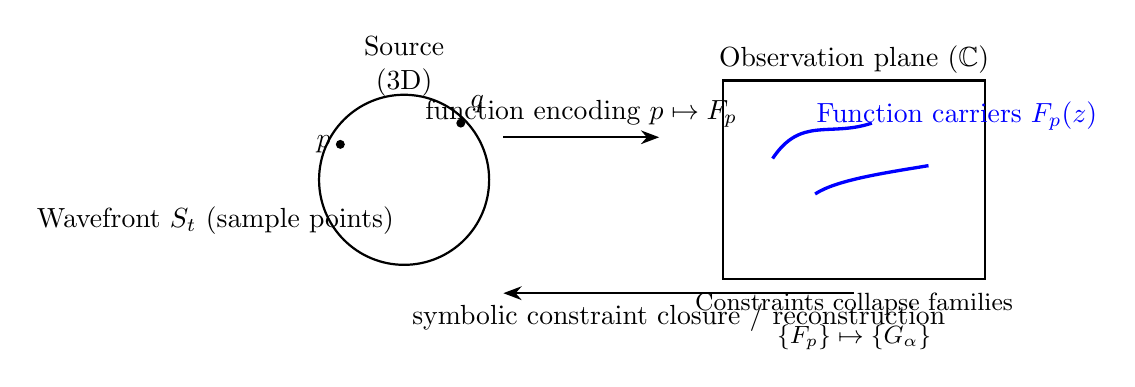
\begin{tikzpicture}[>=Stealth,scale=0.9]
  % R3 sphere on left
  \coordinate (O) at (-3,0);
  \draw[thick] (O) circle (1.2) node[below left,yshift=-6pt] {Wavefront $S_t$ (sample points)};
  % sample points
  \fill ( -3.9,0.5) circle (1.8pt) node[left] {$p$};
  \fill ( -2.2,0.8) circle (1.8pt) node[above right] {$q$};
  % arrow to complex plane
  \draw[->, thick] (-1.6,0.6) -- (0.6,0.6) node[midway,above] {function encoding $p\mapsto F_p$};
  % complex plane rectangle
  \draw[thick] (1.5,-1.4) rectangle (5.2,1.4);
  \node at (3.35,1.7) {Observation plane ($\mathbb{C}$)};
  % sample function carriers
  \draw[blue,very thick] (2.2,0.3) .. controls (2.6,0.9) and (3.0,0.6) .. (3.6,0.8);
  \draw[blue,very thick] (2.8,-0.2) .. controls (3.1,0.0) and (3.8,0.1) .. (4.4,0.2);
  \node[blue] at (4.8,0.9) {Function carriers $F_p(z)$};
  % arrow back (reconstruct)
  \draw[->, thick] (3.35,-1.6) -- (-1.6,-1.6) node[midway,below] {symbolic constraint closure / reconstruction};
  % labels
  \node[align=center] at (-3,1.6) {Source \\ (3D)};
  \node[align=center] at (3.35,-2.0) {\small Constraints collapse families \\ \small $\{F_p\}\mapsto\{G_\alpha\}$};
\end{tikzpicture}
\end{center}


\vspace{8pt}
\noindent\textbf{References \& links.} Full manuscript (Zenodo DOI): \href{https://zenodo.org/records/16904172}{10.5281/zenodo.16904172}.  
Repo / discussion: \url{https://github.com/ndl1971/CEGS-Book./discussions}

\appendix
\section*{Constraint-Induced Functional Geometry}

\noindent To clarify the interpretive meaning of the CEGS mapping 
\[
p \in \mathbb{R}^3 \;\longmapsto\; F_{p}(z) \in \mathcal{F}(\mathbb{C}),
\]
we summarize how constraint operations on the complex function carriers determine the effective geometry recovered when projecting back to physical space.

\medskip
\noindent\textbf{Key Point.} The mapping from $\mathbb{R}^3$ to $\mathbb{C}$ is not a metric projection but a \emph{symbolic encoding}: points in space are represented as complex-valued functions. Constraints (interference conditions, excitation boundaries, propagation rules) act on the \emph{functions}, not on the spatial embedding. Only after constraint closure do we re-introduce spatial interpretation.

\medskip
\noindent This implies a reversal of explanatory order:
\[
\text{(Constraints)} \;\longrightarrow\; \text{(Functional Relations)} \;\longrightarrow\; \text{(Recovered Geometry)}.
\]

\medskip
\noindent Before the result can be stated formally, we introduce a local lemma environment (self-contained):


\begin{lemma}[Constraint-Induced Functional Reorganization]
Let $S_t \subset \mathbb{R}^3$ be a wavefront and let $p \mapsto F_p$ be the CEGS encoding into complex-valued function carriers. If a constraint operator $\mathcal{C}$ acts on the family $\{F_p\}$, producing a collapsed family $\{G_\alpha\}$,
\[
\mathcal{C}:\{F_p\} \longrightarrow \{G_\alpha\},
\]
then the spatial configuration recovered from $\{G_\alpha\}$ after symbolic closure need not coincide with the original spatial embedding of $S_t$. In particular, the recovered geometry is determined by the \emph{functional relations} among $\{G_\alpha\}$, not by the original Euclidean relations among points in $S_t$.
\end{lemma}


\medskip
\noindent\textbf{Interpretation.}  
Interference, diffraction, resonance, and other physical boundary conditions do not alter geometry directly.  
Instead, they \emph{modify the functional relations among the carriers}.  
The geometry observed after reconstruction is therefore:

\[
\textbf{Geometry as an emergent shadow of symbolic constraint closure.}
\]

\medskip
\noindent In this sense:

\begin{itemize}[leftmargin=*,itemsep=4pt]
\item Interference is not merely amplitude overlap; it is the \emph{reorganization of functional identity}.
\item Spatial structure is not primitive; it is \emph{derived}.
\item Geometry is not projected into the complex domain; it is \emph{recovered from it}.
\end{itemize}

\medskip
\noindent Thus the CEGS mapping permits controlled modification of spatial structure by tuning the symbolic interaction of the function carriers, rather than by deforming the underlying Euclidean manifold.



\subsection*{Function Family Coherence}

The constraint-induced geometry in $\mathbb{C}^2$ depends critically on the
choice of the generating oval function family $\mathcal{F}$. 
Each family defines a specific symbolic manifold that determines how
constraints from $\mathbb{R}^3$ are represented after orthogonality lifting.

\begin{lemma}[Function Family Coherence]
Let $\Phi_{\mathcal{F}} : \mathbb{R}^3 \to \mathbb{C}^2$ be a mapping generated by
an oval function family $\mathcal{F} = \{ f_\alpha \}$.
The family $\mathcal{F}$ is coherent with the physical structure of $\mathbb{R}^3$
iff every admissible constraint $\omega$ in $\mathbb{R}^3$ admits a lifted symbolic counterpart
$\tilde{\omega}$ in $\mathbb{C}^2$ such that
\[
\Phi_{\mathcal{F}}^\ast(\tilde{\omega}) \simeq \omega,
\]
where $\simeq$ denotes symbolic equivalence under constraint propagation,
not metric equality.
\end{lemma}

\begin{remark}
This coherence condition ensures that the mapping preserves reconstructibility
without enforcing Euclidean comparability. 
It distinguishes physically meaningful function families from those that violate
the reversibility principle of CEGS.
\end{remark}




This lemma closes the correspondence between constraint-induced structure and
symbolic representation, ensuring that the emergent relations in $\mathbb{C}^2$
are physically admissible and reversible through $\Phi_{\mathcal{F}}^{-1}$.

\section*{Inverse Excitation and Constraint-Based Field Control}
\addcontentsline{toc}{section}{Appendix: Inverse Excitation and Constraint-Based Field Control}

\subsection*{A. Forward Encoding}
Recall that the CEGS wavefront representation assigns to each point \(p \in \mathbb{R}^3\) 
a \emph{function carrier}
\[
F_p : \mathbb{C} \times \mathbb{R} \to \mathbb{C}, \qquad (z,t) \mapsto F_p(z,t),
\]
rather than a scalar projection.  
Let a finite set of controllable emitters be located at points \(x_i \in \mathbb{R}^3\).
Each emitter produces a time-dependent signal \(s_i(t)\).

Wave propagation from \(x_i\) to the observation plane at location \(z \in \mathbb{C}\)
is modeled by a causal Green-type kernel \(G(x_i \to z;\tau)\).  
The induced field carrier is:
\[
F(z,t) \;=\; \sum_{i} \int_{\tau \ge 0} G(x_i \to z;\tau)\, s_i(t-\tau)\, d\tau.
\]
Thus the complete field on the plane is the superposition of symbolic carriers driven by the
source signals.

\subsection*{B. Discretisation and Operator Form}
Discretising time into indices \(k\), plane samples into indices \(j\), and kernels into 
coefficients \(G_{j,i}^{(k-\ell)}\), we obtain the linear operator relation
\[
f_{j,k} = \sum_{i,\ell} G_{j,i}^{(k-\ell)} \, s_{i,\ell}.
\]
Stacking the samples as vectors yields
\[
\mathbf{f} \;=\; \mathbf{A}\,\mathbf{s},
\]
where:
\begin{itemize}[leftmargin=*]
\item \(\mathbf{s}\) is the vector of emitter signals,
\item \(\mathbf{f}\) is the vector of desired field values on the complex plane,
\item \(\mathbf{A}\) encodes propagation, delays, geometry and symbolic carrier relations.
\end{itemize}

\subsection*{C. Inverse Problem (Field Shaping)}
Suppose we wish to \emph{excite a target region} \(R \subset \mathbb{C}\) such that
\[
F(z,t) \approx T(z,t), \qquad z \in R,
\]
for a prescribed time-varying target amplitude \(T\).
In discretised form:
\[
\mathbf{t} \approx \mathbf{A}\mathbf{s}.
\]

We solve the regularised inverse problem
\[
\mathbf{s}^\star
\;=\;
\arg\min_{\mathbf{s}}
\left\| \mathbf{A}\mathbf{s} - \mathbf{t} \right\|^2
+ \lambda \left\| \mathbf{L}\mathbf{s} \right\|^2,
\]
where \(\mathbf{L}\) enforces physical constraints such as:
\begin{itemize}[leftmargin=*]
\item finite bandwidth,
\item causality (\(s_i(t<0)=0\)),
\item amplitude limits of emitters,
\item temporal smoothness if desired.
\end{itemize}

For moderate system size, the solution is explicitly:
\[
\mathbf{s}^\star
=
\big(\mathbf{A}^\top \mathbf{A} + \lambda \mathbf{I}\big)^{-1}
\mathbf{A}^\top \mathbf{t}.
\]

\subsection*{D. Why CEGS Enables This}
Classical optical / wave projection sends each point \(p\in\mathbb{R}^3\) to a \emph{scalar intensity}
at a screen location. This projection is non-invertible: depth, phase and structural coupling are lost.

CEGS replaces this projection by a \emph{function carrier}:
\[
p \mapsto F_p(z,t).
\]

Because each \(F_p\) contains internal algebraic degrees of freedom (phase, local constraint
structure, symbolic generative parameters), the \(\mathbb{R}^3 \to \mathbb{C}\) mapping becomes:
\[
\textbf{reversible up to constraints.}
\]

The key structural feature is:

\begin{lemma}[Orthogonality Lifting]
Internal algebraic orthogonality of complex structure (e.g., \(1 \perp i\)) is preserved,
while Euclidean relational comparability between carriers \(F_p\) and \(F_q\) is deferred.
Relational structure is introduced only through explicit constraints.
\end{lemma}

This deferral enables:
\begin{itemize}[leftmargin=*]
\item symbolic reconfiguration of wave interactions,
\item recoverability of 3D structure from 2D observation,
\item computed excitation control on the plane by shaping emitter signals in space and time.
\end{itemize}

\subsection*{E. Interpretation}
Controlling the field on the complex plane is achieved not by “pushing intensities around,”
but by modifying the symbolic relations among carriers through timed excitation of emitters
in \(\mathbb{R}^3\).  
Interference becomes a form of \emph{symbolic constraint action}.

\bigskip
\noindent
This is precisely where CEGS contributes:
\[
\textit{CEGS converts wave control from geometric projection into symbolic constraint dynamics,}
\]
allowing inversion, recovery, and deliberate shaping of emergent structure.

\vspace{8pt}


\medskip
\noindent
The bidirectional action between excitation (forward) and constraint inversion (feedback)
is elaborated in the following section.



\section*{Potential Applied Context — Field Control via Constraint Inversion}

\noindent
The symbolic mapping \( \mathbb{R}^3 \rightarrow \mathbb{C}^2 \) developed within the CEGS framework
permits reversible correspondence between spatial excitations and emergent field structures.
By representing each point \(p \in \mathbb{R}^3\) as a member of a constraint-governed function family \(F_p(z)\),
excitation and response become linked through symbolic operators rather than direct metric interaction.

\vspace{4pt}
\noindent
In applied settings such as plasma confinement, electromagnetic field shaping, or coherent beam control,
one often seeks to adjust local sources in real space to achieve desired amplitude or phase patterns
in an observation or reaction plane.
The inverse excitation problem can be recast symbolically:
given a desired constraint field \(G(z)\) on the complex domain,
find the corresponding excitation family \(\{F_p\}\) in \(\mathbb{R}^3\) such that
constraint closure under CEGS operators reproduces \(G(z)\) up to symbolic equivalence.

\vspace{4pt}
\noindent
This inversion operates without assuming Euclidean comparability between \(F_p\) and \(F_q\);
metric relations re-emerge only as a consequence of constraint resolution.
Thus, excitation planning becomes a process of symbolic feedback:
constraints defined in the complex domain prescribe transformations in the real domain,
and vice versa, through reversible functional correspondence.

\vspace{4pt}
\noindent
Such a formulation offers a new analytic handle for field control problems:
\begin{itemize}[leftmargin=*,itemsep=4pt]
  \item \emph{Predictive modeling:} symbolic inversion may reveal stable or resonant excitation geometries
        without full numeric field simulation.
  \item \emph{Feedback design:} constraint propagation between domains provides a direct pathway
        for adaptive field correction and optimization.
  \item \emph{Unified abstraction:} excitation, propagation, and observation appear as
        algebraically coupled layers within a single symbolic system,
        aligning physical constraints with generative mathematical structure.
\end{itemize}

\vspace{4pt}
\noindent
In this sense, CEGS supplies a general symbolic calculus for emergent field behavior:
a framework where excitation design, constraint feedback, and field stabilization
are expressed not as numerical boundary problems but as
symbolic transformations between generative domains.

\vspace{10pt}
\begin{center}
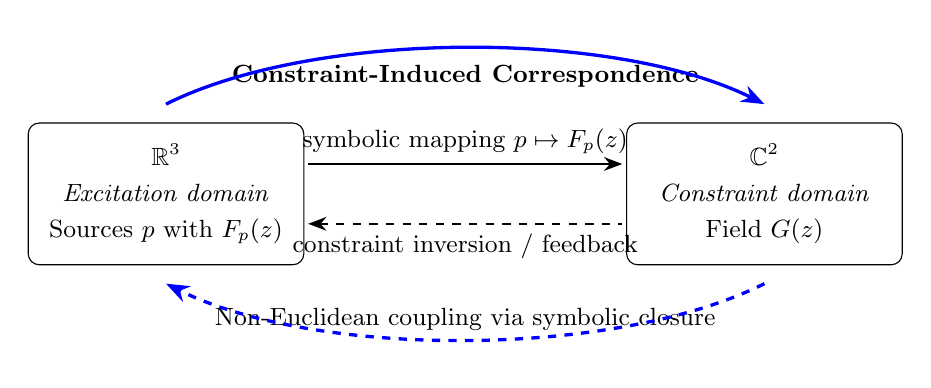
\begin{tikzpicture}[>=Stealth,scale=0.95, every node/.style={font=\small}]
  % Domains
  \node[draw,rounded corners,minimum width=3.5cm,minimum height=1.8cm,align=center] (R3) at (-4,0)
    {$\mathbb{R}^3$ \\[2pt] \emph{Excitation domain}\\[2pt] Sources $p$ with $F_p(z)$};
  \node[draw,rounded corners,minimum width=3.5cm,minimum height=1.8cm,align=center] (C2) at (4,0)
    {$\mathbb{C}^2$ \\[2pt] \emph{Constraint domain}\\[2pt] Field $G(z)$};

  % Forward map
  \draw[->, thick] (-2.1,0.4) -- (2.1,0.4)
    node[midway,above] {symbolic mapping $p \mapsto F_p(z)$};

  % Inverse constraint feedback
  \draw[<-, thick,dashed] (-2.1,-0.4) -- (2.1,-0.4)
    node[midway,below] {constraint inversion / feedback};

  % Annotations
  \node[align=center,anchor=south] at (0,1.3)
    {\textbf{Constraint-Induced Correspondence}};
  \node[align=center,anchor=north] at (0,-1.4)
    {Non-Euclidean coupling via symbolic closure};

  % Decorative arrows
  \draw[blue,very thick,->] (-4,1.2) .. controls (-2,2.2) and (2,2.2) .. (4,1.2);
  \draw[blue,very thick,->,dashed] (4,-1.2) .. controls (2,-2.2) and (-2,-2.2) .. (-4,-1.2);
\end{tikzpicture}

\vspace{6pt}
\textit{Figure: Bidirectional correspondence between real-space excitations in $\mathbb{R}^3$
and constraint fields in $\mathbb{C}^2$. Solid arrows denote forward symbolic encoding,
dashed arrows denote inverse constraint feedback.}
\end{center}

\section*{Practical Recipe: Inverse Excitation for a Simple Aperture Geometry}
\addcontentsline{toc}{section}{Practical Recipe: Inverse Excitation}

We summarise a concrete five-step procedure to compute real-space emitter signals
that produce a desired time-dependent excitation on the observation plane under
the CEGS encoding. The example geometry is a single planar aperture (observation
plane) and two point emitters in $\mathbb{R}^3$.

\subsection*{1. Geometry}
Let the observation plane (screen) be the plane $z = z_0$ in Cartesian coordinates.
Define two point emitters at positions $x_1=(x_{1},y_{1},z_{s})$ and
$x_2=(x_{2},y_{2},z_{s})$ with $z_s<z_0$. The aperture is the disk
\[
P = \{ (x,y,z_0) : x^2 + y^2 \le R^2 \}.
\]
Choose an observation grid on $P$ with points $z_j\in P$, $j=1,\dots,N_p$.

\subsection*{2. Forward Green's kernel (free space)}
For homogeneous free-space wave propagation (scalar wave, speed $c$), the causal
impulse response from emitter at $x_i$ to location $z$ on the plane is given by the
retarded Green's function (distributional):
\[
G(x_i \to z; \tau) \;=\; \frac{\delta\!\big(\tau - \tfrac{\|z-x_i\|}{c}\big)}{4\pi \|z-x_i\|}.
\]
For narrowband or time-harmonic signals $s_i(t)=\Re\{ \tilde{s}_i e^{-\mathrm{i}\omega t}\}$,
the frequency-domain transfer is
\[
\hat{G}(x_i\to z;\omega) \;=\; \frac{e^{-\mathrm{i}\omega \|z-x_i\|/c}}{4\pi \|z-x_i\|}.
\]
Use the time-domain Green's form for transient control or the frequency-domain form
for band-limited design.

\subsection*{3. Discretisation}
Discretise time into samples $t_k = k\Delta t$ for $k=0,\dots,K-1$ and the aperture
plane into $N_p$ sample points $z_j$. Discretise source signals $s_{i}(t)$ into
samples $s_{i,\ell}$.

A sampled forward model is:
\[
f_{j,k} \;=\; \sum_{i=1}^{2} \sum_{\ell=0}^{K-1} G_{j,i}^{(k-\ell)}\, s_{i,\ell},
\]
where $G_{j,i}^{(m)}$ denotes the sampled kernel with delay index $m$:
\[
G_{j,i}^{(m)} \approx \int_{m\Delta t}^{(m+1)\Delta t} G(x_i\to z_j;\tau)\, d\tau.
\]
Stack the unknown source vector $\mathbf{s}\in\mathbb{R}^{2K}$ by concatenating
each emitter's $K$ time samples; stack field samples $\mathbf{f}\in\mathbb{R}^{N_pK}$.
Then
\[
\mathbf{f} = \mathbf{A}\,\mathbf{s},
\]
where $\mathbf{A}\in\mathbb{R}^{N_pK\times 2K}$ is constructed from the $G_{j,i}^{(m)}$.

\subsection*{4. Inversion: Tikhonov with causality \& bandlimit}
Specify a target $\mathbf{t}$ containing desired samples $T(z_j,t_k)$ on selected
plane region $R\subset P$ and time window. We solve:
\[
\mathbf{s}^\star
\;=\;
\arg\min_{\mathbf{s}}
\;\;
\|\mathbf{W}(\mathbf{A}\mathbf{s}-\mathbf{t})\|_2^2
\;+\;\lambda\|\mathbf{L}\mathbf{s}\|_2^2,
\]
where:
\begin{itemize}
  \item $\mathbf{W}$ is a diagonal weighting (causal mask and region mask) that zeros
        out unwanted plane/time entries (enforcing the target region and time window);
  \item $\mathbf{L}$ enforces smoothness or spectral constraints (e.g. discrete
        time-difference operator to suppress high-frequency components);
  \item $\lambda>0$ is the regularisation parameter.
\end{itemize}

\noindent\textbf{Causality enforcement.} Set $s_{i,\ell}=0$ for $\ell<0$ and, if needed,
add inequality constraints to prevent pre-emission; in discrete Tikhonov this is
enforced by construction (we only include $\ell$ within $[0,K-1]$).

\noindent\textbf{Bandlimit enforcement.} Either (a) include $\mathbf{L}$ as a high-pass
penalty (large weight on high-frequency components), or (b) formulate and solve the
problem in the frequency domain and restrict to frequencies $\omega\in[\omega_{\min},\omega_{\max}]$.

\noindent\textbf{Closed-form (small systems).} The Tikhonov solution is:
\[
\mathbf{s}^\star = (\mathbf{A}^\top\mathbf{W}^\top\mathbf{W}\mathbf{A} + \lambda \mathbf{L}^\top\mathbf{L})^{-1}
\mathbf{A}^\top\mathbf{W}^\top\mathbf{W}\mathbf{t}.
\]

For large systems use iterative solvers (LSQR, conjugate gradient on normal eqns)
with matrix-vector products implemented by fast evaluation of $\mathbf{A}\mathbf{s}$
and $\mathbf{A}^\top \mathbf{v}$ without forming $\mathbf{A}$ explicitly.

\subsection*{5. Validation and refinement: forward simulation, adjoint loops, time-reversal}
\begin{enumerate}[leftmargin=*,itemsep=4pt]
  \item \textbf{Forward simulate:} compute $\mathbf{f}_{\rm sim} = \mathbf{A}\mathbf{s}^\star$,
        compare to $\mathbf{t}$ on the target region via RMSE or other metric.
  \item \textbf{Adjoint refinement:} compute the residual $\mathbf{r}=\mathbf{W}(\mathbf{f}_{\rm sim}-\mathbf{t})$
        and update sources by gradient steps using the adjoint $\mathbf{A}^\top$:
        \[
        \mathbf{s}_{n+1} = \mathbf{s}_n - \eta [\mathbf{A}^\top(\mathbf{W}^\top\mathbf{W}(\mathbf{A}\mathbf{s}_n-\mathbf{t}))
        + \lambda \mathbf{L}^\top\mathbf{L}\mathbf{s}_n].
        \]
        Choose step size $\eta$ by backtracking or Armijo rule.
  \item \textbf{Time-reversal (experimental / robust):}
        If direct measurement is possible, place a virtual probe at the target pattern,
        record the fields at the emitter locations, time-reverse those recordings and
        play back — this naturally focuses energy at the desired region and is robust
        to medium uncertainty.
  \item \textbf{Iterate:} use the measured forward response (or updated simulated kernel)
        to re-solve the inverse problem until convergence.
\end{enumerate}

\subsection*{Implementation notes and recommended parameters}
\begin{itemize}[leftmargin=*]
  \item \textbf{Sampling:} choose $\Delta t$ small enough to sample the highest frequency of interest
        (Nyquist). For optical-like examples this becomes demanding; prefer microwave/sonic examples for initial tests.
  \item \textbf{Grid:} $N_p$ should balance resolution vs computational cost. Start coarse (e.g. $N_p\sim 1000$) then refine.
  \item \textbf{Regularisation $\lambda$:} choose by L-curve or cross-validation. Start with a small value (e.g. $10^{-6}\!-\!10^{-3}$) and scale by condition number heuristics.
  \item \textbf{Solvers:} LSQR or Conjugate Gradient are recommended for large sparse systems; use preconditioning if available.
  \item \textbf{Robustness:} if $G$ is uncertain, include model-error penalties or use time-reversal based calibration.
\end{itemize}

\subsection*{Algorithm (pseudocode)}
\begin{verbatim}
1. Define geometry: emitter positions x1, x2; plane grid {z_j}; time grid {t_k}
2. Compute kernel samples G_{j,i}^{(m)} from Green formula (or measure)
3. Build operator A (explicitly or as mat-vec rules)
4. Define target vector t on chosen region/time window
5. Choose weights W, regulariser L, parameter lambda
6. Solve for s* via iterative Tikhonov (LSQR) or closed-form if small
7. Simulate f_sim = A s*
8. If error acceptable -> done. Else:
   a) compute residual r = W (f_sim - t)
   b) gradient step s <- s - eta*(A^T(W^T W r) + lambda L^T L s)
   c) repeat steps 7-8, or run time-reversal calibration
\end{verbatim}

\noindent This recipe provides a direct implementation path from the symbolic CEGS
field-target specification to physically executable emitter signals in $\mathbb{R}^3$.


\section*{Worked Example: Circular Aperture, Two Emitters (Fresnel Approximation)}
\addcontentsline{toc}{section}{Worked Example: Circular Aperture, Two Emitters}

This worked example demonstrates the five-step recipe in a compact analytic setting.
We choose a circular observation aperture, two point emitters, and use a Fresnel
(small-angle) approximation for the free-space Green kernel to obtain an explicit
forward operator suitable for a small-scale Tikhonov test problem.

\subsection*{Geometry and parameters}
Let the observation (aperture) plane be \(z=z_0\). The aperture is the disk
\[
P=\{(x,y,z_0): x^2+y^2\le R^2\}.
\]
Two point emitters are placed on the axis at
\[
x_1=(d,0,0),\qquad x_2=(-d,0,0),
\]
with emitter plane \(z=0\) and \(0<d\ll z_0\). The speed of propagation is \(c\)
and the (dominant) angular frequency is \(\omega\) (wavelength \(\lambda=2\pi c/\omega\)).

For the worked numeric illustration choose (example values):
\[
R = 0.05\ \text{m},\quad z_0 = 0.5\ \text{m},\quad d = 0.02\ \text{m},\quad
\lambda = 0.01\ \text{m}.
\]

\subsection*{Fresnel (paraxial) kernel}
Under the small-angle (Fresnel/paraxial) approximation the time-harmonic Green's
function from emitter \(x_i=(x_{i},y_{i},0)\) to plane point \(z=(x,y,z_0)\) is
approximated by
\[
\hat{G}(x_i\to z;\omega) \approx \frac{e^{-\mathrm{i}k z_0}}{4\pi z_0}
\exp\!\Big(-\mathrm{i}\frac{k}{2z_0}\big[(x-x_i)^2 + (y-y_i)^2\big]\Big),
\]
where \(k=\tfrac{2\pi}{\lambda}\) is the wavenumber. The common phase factor
\(e^{-\mathrm{i}k z_0}/(4\pi z_0)\) may be absorbed into amplitude scaling.

For pulsed / transient design one may inverse-Fourier-transform the above or
use a discrete narrowband approximation; here we demonstrate narrowband control.

\subsection*{Discrete sampling (tiny illustrative system)}
Select a coarse sampling of the aperture with \(N_p=4\) points (toy example)
arranged symmetrically on the disk:
\[
z_1=(r,0,z_0),\quad z_2=(-r,0,z_0),\quad z_3=(0,r,z_0),\quad z_4=(0,-r,z_0),
\]
with \(r=R/2\). Use a small temporal discretisation with a single narrowband
time-slice (so we work in frequency-domain complex amplitudes). Denote emitter
complex phasors by \(\tilde{s}_1,\tilde{s}_2\), and measured complex amplitudes
on the aperture by \(\tilde{f}_j\) for \(j=1,\dots,4\).

Using the Fresnel kernel, the sampled forward model is:
\[
\tilde{f}_j \;=\; \sum_{i=1}^2 \hat{G}_{j,i}\,\tilde{s}_i,
\qquad
\hat{G}_{j,i} \;=\; \exp\!\Big(-\mathrm{i}\frac{k}{2z_0}\|p_j - x_i\|^2\Big),
\]
where \(p_j=(x_j,y_j, z_0)\) denotes the \(j\)-th aperture sample (we drop the common
amplitude prefactor for simplicity).

Stacking \(\tilde{\mathbf{f}}=(\tilde{f}_1,\dots,\tilde{f}_4)^\top\) and
\(\tilde{\mathbf{s}}=(\tilde{s}_1,\tilde{s}_2)^\top\) yields
\[
\tilde{\mathbf{f}} = \mathbf{\hat{G}}\,\tilde{\mathbf{s}},
\]
with \(\mathbf{\hat{G}}\in\mathbb{C}^{4\times 2}\) the sampled transfer matrix.

\subsection*{Target pattern}
Choose a simple target: double amplitude on the right half of the aperture,
i.e. a desired complex vector \(\tilde{\mathbf{t}}\) proportional to
\((2,1,2,1)^\top\) (phase chosen zero for simplicity). Normalise so the target
has moderate total energy.

\subsection*{Tikhonov inversion (closed-form for tiny system)}
Solve the regularised least-squares problem (frequency-domain narrowband):
\[
\tilde{\mathbf{s}}^\star
=\arg\min_{\tilde{\mathbf{s}}}
\;\; \|\mathbf{\hat{G}}\tilde{\mathbf{s}} - \tilde{\mathbf{t}}\|_2^2
+ \lambda \|\tilde{\mathbf{s}}\|_2^2.
\]
For this small system the closed-form solution is:
\[
\tilde{\mathbf{s}}^\star
= (\mathbf{\hat{G}}^\dagger \mathbf{\hat{G}} + \lambda \mathbf{I})^{-1}
\mathbf{\hat{G}}^\dagger \tilde{\mathbf{t}},
\]
where \(\mathbf{\hat{G}}^\dagger\) denotes the Hermitian transpose.

\paragraph{Illustrative numeric step.} Compute \(\mathbf{\hat{G}}\) with the
chosen parameters (\(k\) from \(\lambda=0.01\) m, \(z_0=0.5\) m, emitter offsets
\(\pm d\)). With \(\lambda\) small (e.g. \(\lambda=10^{-3}\)) the resulting
\(\tilde{\mathbf{s}}^\star\) gives the complex amplitudes for the two emitters
that best approximate the target pattern in least-squares sense.

\subsection*{Forward validation}
Compute the simulated aperture response \(\tilde{\mathbf{f}}_{\rm sim}=
\mathbf{\hat{G}}\tilde{\mathbf{s}}^\star\) and evaluate the relative error:
\[
\mathrm{RMSE} = \frac{\|\tilde{\mathbf{f}}_{\rm sim} - \tilde{\mathbf{t}}\|_2}
{\|\tilde{\mathbf{t}}\|_2}.
\]
If RMSE is acceptable (e.g. \(<0.1\)) the design is successful for the coarse test;
otherwise, refine by increasing sampling density, reducing \(\lambda\) (with care),
or using an iterative adjoint update.

\subsection*{Adjoint refinement (one gradient step)}
Compute residual \(\mathbf{r}=\mathbf{\hat{G}}\tilde{\mathbf{s}}^\star - \tilde{\mathbf{t}}\)
and perform a single adjoint update with step-size \(\eta\):
\[
\tilde{\mathbf{s}} \leftarrow \tilde{\mathbf{s}}^\star - \eta\,
\mathbf{\hat{G}}^\dagger \mathbf{r}.
\]
Choose \(\eta\) small (line-search or \(\eta\approx 10^{-2}\)) and repeat forward
simulation until convergence.

\subsection*{Remarks}
\begin{itemize}[leftmargin=*]
  \item The Fresnel approximation yields a compact, phase-only kernel that is easy to
        evaluate and sufficient for small-angle setups. For wide-angle or near-field
        scenarios use the full retarded Green function.
  \item The toy \(4\times 2\) example illustrates the inversion algebraically.
        For realistic experiments use denser spatial/time sampling and iterative
        solvers (LSQR, CG) with preconditioning.
  \item To enforce causality and time-domain bandlimits one repeats the above in
        the time-domain with convolutional kernels \(G_{j,i}^{(m)}\) as in the main text.
\end{itemize}

\noindent This worked example demonstrates how CEGS' function-carrier viewpoint
naturally integrates with classical Fresnel optics and standard inverse methods,
producing a compact, implementable inversion for emitter synthesis.

\subsection*{Worked Example — Numerical Results (Fresnel toy)}
Using the parameters from the Fresnel worked example:
\[
R=0.05\ \text{m},\quad z_0=0.5\ \text{m},\quad d=0.02\ \text{m},\quad \lambda=0.01\ \text{m},
\quad r=R/2=0.025\ \text{m},
\]
and the four sampling points
\[
p_1=(r,0,z_0),\ p_2=(-r,0,z_0),\ p_3=(0,r,z_0),\ p_4=(0,-r,z_0),
\]
with two emitters \(x_1=(d,0,0),\,x_2=(-d,0,0)\), we compute the sampled
Fresnel transfer matrix \(\hat{\mathbf{G}}\in\mathbb{C}^{4\times 2}\).
With \(k=2\pi/\lambda\) the numeric matrices/vectors are:

\[
k \;=\; 628.3185307179587.
\]

\[
\hat{\mathbf{G}} \;=\;
\begin{bmatrix}
0.999877 - 0.015707\,\mathrm{i} & 0.294040 - 0.955793\,\mathrm{i} \\
0.294040 - 0.955793\,\mathrm{i} & 0.999877 - 0.015707\,\mathrm{i} \\
0.799685 - 0.600420\,\mathrm{i} & 0.799685 - 0.600420\,\mathrm{i} \\
0.799685 - 0.600420\,\mathrm{i} & 0.799685 - 0.600420\,\mathrm{i}
\end{bmatrix}.
\]

The (normalized) target vector chosen proportional to \((2,1,2,1)^\top\) is

\[
\tilde{\mathbf{t}} \;=\; \frac{1}{\sqrt{10}}(2,1,2,1)^\top
\;=\;
\begin{bmatrix}0.632456\\[2pt] 0.316228\\[2pt] 0.632456\\[2pt] 0.316228\end{bmatrix}.
\]

We use Tikhonov regularisation with \(\lambda_{\rm reg}=10^{-3}\).
Compute \(\tilde{\mathbf{s}}^\star = (\hat{\mathbf{G}}^\dagger\hat{\mathbf{G}}+\lambda_{\rm reg}\mathbf{I})^{-1}\hat{\mathbf{G}}^\dagger\tilde{\mathbf{t}}\).
Numerically we obtain the source phasors:

\[
\tilde{\mathbf{s}}^\star \approx
\begin{bmatrix}
0.28804 + 0.04820\,\mathrm{i} \\
0.12664 + 0.26316\,\mathrm{i}
\end{bmatrix}.
\]

The simulated aperture response is
\[
\tilde{\mathbf{f}}_{\rm sim} = \hat{\mathbf{G}}\tilde{\mathbf{s}}^\star
\approx
\begin{bmatrix}
0.577524 + 0.000000\,\mathrm{i} \\
0.261525 - 0.000000\,\mathrm{i} \\
0.518560 + 0.000000\,\mathrm{i} \\
0.518560 + 0.000000\,\mathrm{i}
\end{bmatrix}.
\]

The relative root-mean-square error (RMSE) relative to the target is
\[
\mathrm{RMSE} \;=\; \frac{\|\tilde{\mathbf{f}}_{\rm sim} - \tilde{\mathbf{t}}\|_2}{\|\tilde{\mathbf{t}}\|_2}
\;\approx\; 0.2448.
\]

\paragraph{Interpretation.}
\begin{itemize}[leftmargin=*,itemsep=4pt]
  \item The toy two-emitter, four-sample system reconstructs the target pattern only approximately (RMSE about 24\%). This is expected for an extremely undersampled test case.
  \item The computed source phasors show both amplitude and phase adjustments: in general both are required to shape the complex-plane pattern.
  \item Improvements (lower RMSE) are achieved by: increasing aperture sampling \(N_p\), adding more controllable emitters, tuning \(\lambda_{\rm reg}\) via L-curve/cross-validation, or switching to a time-domain design with richer temporal degrees of freedom.
  \item Time-reversal or adjoint iterative refinement (as described in the recipe) are practical next steps to calibrate against model mismatch and medium uncertainty.
\end{itemize}

\paragraph{Suggested immediate refinements for a next run}
\begin{enumerate}[leftmargin=*,itemsep=4pt]
  \item Increase the number of aperture samples (e.g. 16 or 64 points) to reduce aliasing and better resolve spatial patterns.
  \item Add at least one or two additional emitters (off-axis) to enlarge the control space.
  \item Sweep \(\lambda_{\rm reg}\) (L-curve) to find the best tradeoff between fitting and stability.
  \item If possible measure or numerically simulate the full time-domain Green kernels and perform a time-domain inversion (convolutional Tikhonov), which typically yields richer control and causality enforcement.
\end{enumerate}

\paragraph{Conditioning of the Inversion.}
The ill-conditioning of the inverse problem can be directly inspected
from the normal matrix
\[
\hat{\mathbf{N}} \;=\; \hat{\mathbf{G}}^\dagger \hat{\mathbf{G}}
\;=\;
\begin{bmatrix}
2.5208 - 0.0000\,\mathrm{i} & 1.8366 - 0.0296\,\mathrm{i} \\[4pt]
1.8366 + 0.0296\,\mathrm{i} & 2.5208 + 0.0000\,\mathrm{i}
\end{bmatrix}.
\]
Its eigenvalues are
\[
\lambda_1 \approx 4.348, \qquad
\lambda_2 \approx 0.694.
\]
Hence the condition number is
\[
\kappa(\hat{\mathbf{N}}) = \frac{\lambda_1}{\lambda_2} \approx 6.27,
\]
indicating a moderately ill-conditioned system: small perturbations in
the measured amplitudes or numerical noise can produce up to a factor of
six amplification in the reconstructed source coefficients.

Adding the Tikhonov term \(\lambda_{\mathrm{reg}}\mathbf{I}\)
shifts the eigenvalues to
\(\lambda'_i = \lambda_i + \lambda_{\mathrm{reg}}\),
which stabilises the inversion while slightly biasing the amplitude.
For the present toy value
\(\lambda_{\mathrm{reg}} = 10^{-3}\),
the shift is negligible but sufficient to regularise the matrix inverse.

\paragraph{Discussion.}
Condition-number analysis highlights the geometric intuition behind
constraint inversion:
if the sampled fields at the aperture are nearly collinear in
\(\mathbb{C}^N\), then the Gram matrix becomes singular and control
over independent spatial modes is lost.
In CEGS terminology, this corresponds to a local collapse of the
functional degrees of freedom within the complex projection manifold.
Ensuring a well-conditioned mapping thus requires sufficiently distinct
sampling functions (emitters, phases, or temporal encodings).

\paragraph{Visualising Stability Domains.}

A practical way to understand constraint inversion is to examine how the
conditioning of the projection operator varies with geometry or
wavelength.  
Let the emitter separation be \(d\), and define the wavelength
\(\lambda\).  
The entries of the Green’s matrix
\(\hat{\mathbf{G}}(d,\lambda)\)
depend on the phase difference
\(\Delta \phi = 2\pi d / \lambda\).
For each pair \((d,\lambda)\),
the normal matrix
\(\hat{\mathbf{N}} = \hat{\mathbf{G}}^\dagger \hat{\mathbf{G}}\)
can be diagonalised to obtain the singular values
\(\sigma_1(d,\lambda)\) and \(\sigma_2(d,\lambda)\).

\[
\kappa(d,\lambda)
  = \frac{\sigma_{\max}(d,\lambda)}{\sigma_{\min}(d,\lambda)}
  = \frac{\sigma_1(d,\lambda)}{\sigma_2(d,\lambda)}.
\]

Plotting \(\kappa(d,\lambda)\) yields a *stability map*:
regions where \(\kappa \approx 1\) correspond to well-conditioned
geometries (independent functional modes),
while ridges of large \(\kappa\) indicate *degenerate configurations*
where the emitters become phase-aligned and symbolic reconstruction
loses independence.

\vspace{6pt}
\noindent
In the CEGS framework, this stability landscape is interpreted as a
measure of *functional separation* between emitters in
\(\mathbb{C}^2\).  
A configuration with low condition number corresponds to a
wavefront ensemble whose lifted functions
\(\{F_p(z)\}\)
span a near-orthogonal basis on the complex plane,
enabling fine-grained constraint control and reversible excitation.
High condition-number regions correspond to symbolic collapse:
different emitters map to nearly the same constraint path, and
inverse excitation becomes unstable or non-unique.

\begin{center}
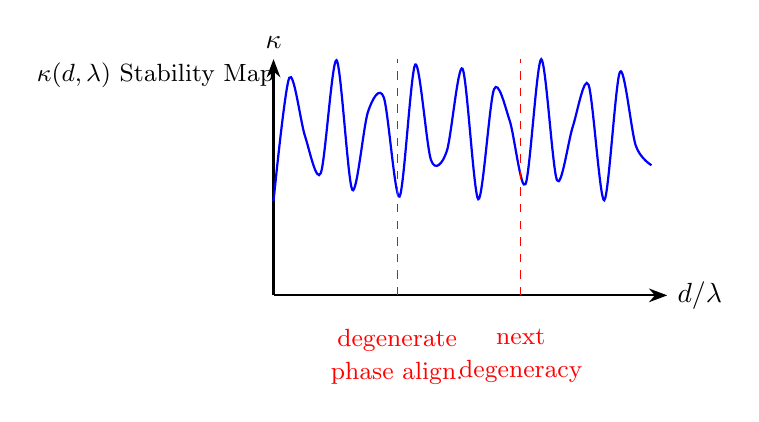
\begin{tikzpicture}[>=Stealth,scale=1.0]
  \node at (-1.5,2.8) {\small $\kappa(d,\lambda)$ Stability Map};
  \draw[thick,->] (0,0) -- (5,0) node[right] {$d / \lambda$};
  \draw[thick,->] (0,0) -- (0,3) node[above] {$\kappa$};
  \draw[domain=0:4.8,smooth,variable=\x,thick,blue]
        plot ({\x},{1.2+1.8*sin(6*\x r)^2});
  \draw[dashed,red] (1.57,0) -- (1.57,3);
  \draw[dashed,red] (3.14,0) -- (3.14,3);
  \node[red,align=center,below] at (1.57,-0.3)
        {\small degenerate\\\small phase align.};
  \node[red,align=center,below] at (3.14,-0.3)
        {\small next\\\small degeneracy};
\end{tikzpicture}
\end{center}

\paragraph{Interpretation.}
This schematic shows how emitter separation relative to wavelength
controls the symbolic independence of the complex function family.
By tuning \(d/\lambda\) away from degeneracy lines,
the mapping \(\mathbb{R}^3 \to \mathbb{C}^2\)
remains stable under constraint inversion, allowing controlled
inverse excitation of specific planar regions.

\paragraph{Summary.}
\begin{itemize}
  \item The condition number \(\kappa(d,\lambda)\) quantifies how well
        the lifted functions span the target complex manifold.
  \item Low \(\kappa\) (blue valleys) $\Rightarrow$ robust reconstruction.
  \item High \(\kappa\) (red ridges) $\Rightarrow$ functional collapse.
  \item Practical tuning of emitter geometry or constraint timing
        can thus be viewed as *navigating the stability manifold* in
        \((d,\lambda)\)-space.
\end{itemize}

\section*{Domain Partitioning under Multiple Generators}

When several independent emitters or generative sources are active within the same geometric field, the mapping 
\(\mathbb{R}^3 \rightarrow \mathbb{C}\)
produces overlapping functional domains on the observation plane.
Each emitter \(E_i\) defines a family of complex functions
\[
F^{(i)}_p : \mathbb{C} \to \mathbb{C}, \qquad
F^{(i)}_p(z) = A^{(i)}_p(z)\, e^{\mathrm{i}\Phi^{(i)}_p(z)},
\]
which encode the symbolic amplitude--phase structure of the wavefront generated by the point \(p \in \mathbb{R}^3\)
belonging to that source.

\paragraph{Single-emitter domains.}
In regions of the complex plane where one function family dominates
(\(|F^{(i)}(z)| \gg |F^{(j)}(z)|\) for all \(j\neq i\)),
the symbolic structure is locally determined by a single constraint set.
Such domains represent \emph{simple closures} in the CEGS sense:
constraint satisfaction occurs within one generator’s algebraic framework.
These areas correspond physically to coherent, non-interfering projection zones of an individual source.

\paragraph{Co-constrained or interference domains.}
Where two or more families overlap, the observable field is a superposition
\[
G(z) = \sum_i F^{(i)}(z),
\]
and the governing constraints act jointly across emitters.
These regions are \emph{composite closures}:
multiple constraint sets must be satisfied simultaneously.
Their interaction gives rise to emergent patterns---interference fringes, bifurcation lines,
and other structures where symbolic relations between phase, amplitude, and constraint operators
collapse or reinforce one another.
Such domains are where CEGS reveals structure that classical projection
would regard merely as destructive or constructive interference.

\paragraph{Constraint topology.}
The partition of the observation plane into single-emitter and co-constrained regions
defines a symbolic topology of influence:
\[
\Omega = \bigcup_i \Omega_i^{(1)} \;\cup\; \bigcup_{i<j} \Omega_{ij}^{(2)} \;\cup\; \cdots
\]
where \(\Omega_i^{(1)}\) denotes single-emitter domains
and \(\Omega_{ij}^{(2)}\) the pairwise interference domains.
Constraint operators act differently on each class,
and their algebraic composition determines how information flows
between generators and the observed symbolic field.

\paragraph{Interpretation.}
This decomposition clarifies why the CEGS mapping is valuable:
by lifting Euclidean relational constraints, one can study symbolic regions
under distinct constraint regimes rather than relying on metric overlap alone.
Subsequent sections, such as \emph{Inverse Excitation and Constraint-Based Field Control},
leverage this structure to compute how controlled excitations in \(\mathbb{R}^3\)
can target, modify, or stabilize specific regions in the complex field.


\begin{center}
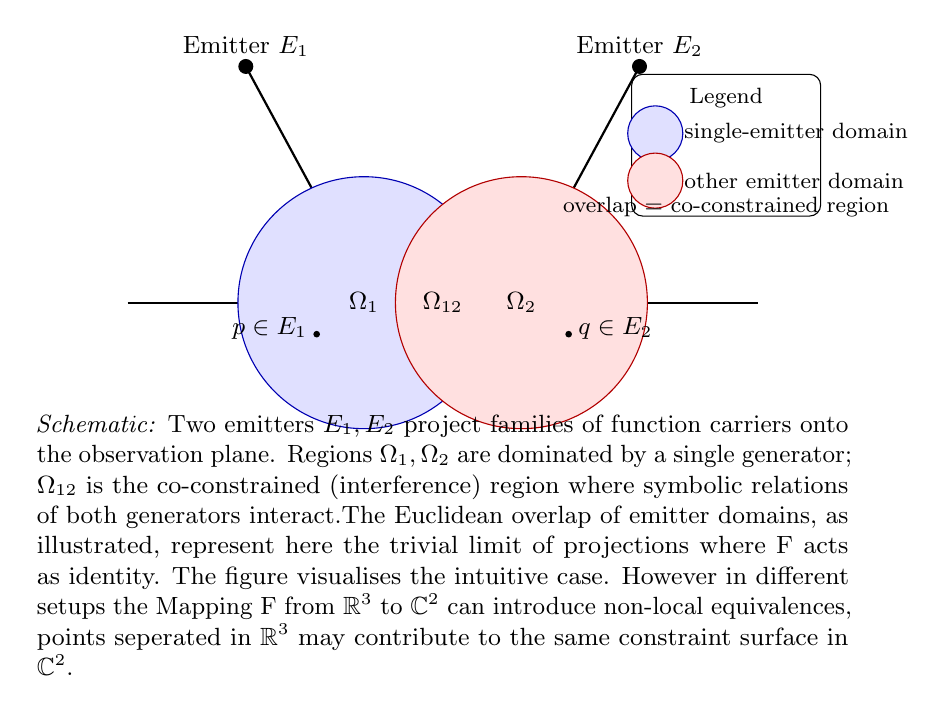
\begin{tikzpicture}[every node/.style={font=\small}, scale=1]
  % Define coordinates
  \coordinate (E1) at (-2.5,2.2); % emitter 1
  \coordinate (E2) at ( 2.5,2.2); % emitter 2
  \coordinate (P)  at (0,0);      % center of plane

  % Draw observation plane
  \draw[thick] (-4,-0.8) -- (4,-0.8);
  \node[below] at (0,-0.8) {Observation plane ($\mathbb{C}$)};

  % Draw emitters (points above plane)
  \filldraw[black] (E1) circle (2.5pt) node[above] {Emitter $E_1$};
  \filldraw[black] (E2) circle (2.5pt) node[above] {Emitter $E_2$};

  % Arrows from emitters to plane
  \draw[->, thick] (E1) -- (-1.2,-0.2) node[midway, left] {};
  \draw[->, thick] (E2) -- ( 1.2,-0.2) node[midway, right] {};

  % Draw single-emitter domains (overlapping circles on plane)
  \filldraw[fill=blue!12, draw=blue!70!black] (-1.0,-0.8) circle (1.6cm);
  \filldraw[fill=red!12,  draw=red!70!black]  ( 1.0,-0.8) circle (1.6cm);

  % Labels for domains
  \node at (-1.0,-0.8)    {$\Omega_1$};
  \node at ( 1.0,-0.8)    {$\Omega_2$};
  \node at ( 0.0,-0.8)    {$\Omega_{12}$};

  % Draw small sample points and arrows indicating mapping p -> F_p(z)
  \fill ( -1.6,-1.2) circle (1.2pt) node[left,yshift=2pt] {$p\in E_1$};
  \fill (  1.6,-1.2) circle (1.2pt) node[right,yshift=2pt] {$q\in E_2$};

  % Legend box
  \begin{scope}[shift={(3.6,1.2)}]
    \draw[rounded corners,thin] (-1.2,-0.9) rectangle (1.2,0.9);
    \node at (0,0.6) {\footnotesize Legend};
    \filldraw[fill=blue!12,draw=blue!70!black] (-0.9,0.15) circle (0.35cm) node[right,xshift=7pt] {\footnotesize single-emitter domain};
    \filldraw[fill=red!12, draw=red!70!black]  (-0.9,-0.45) circle (0.35cm) node[right,xshift=7pt] {\footnotesize other emitter domain};
    \node at (0,-0.78) {\footnotesize overlap = co-constrained region};
  \end{scope}

  % caption-like note
  \node[below,align=center] at (0,-2.1) {\parbox{0.85\textwidth}{\small\textit{Schematic:} Two emitters $E_1,E_2$ project families of function carriers onto the observation plane. Regions $\Omega_1,\Omega_2$ are dominated by a single generator; $\Omega_{12}$ is the co-constrained (interference) region where symbolic relations of both generators interact.The Euclidean overlap of emitter domains, as illustrated, represent here the trivial limit of projections where F acts as identity. The figure visualises the intuitive case. However in different setups the Mapping F from $\mathbb{R}^3$ to $\mathbb{C}^2$ can introduce non-local equivalences, points seperated in $\mathbb{R}^3$ may contribute to the same constraint surface in  $\mathbb{C}^2$. }};
\end{tikzpicture}
\end{center}


\section*{Representative Real-World Examples Where CEGS Excels}

\subsection*{(1) Phase-Conjugate / Mirror-Symmetric Emitters}
Phase-conjugation and mirror-symmetric emitter arrangements (for example in nonlinear
optics with phase-conjugate mirrors) produce wavefronts whose phase relationships
are inverted or mirrored. In classical descriptions, a medium or nonlinear process
is required to couple separated wavefront pieces. Under CEGS, such coupling can be
seen as a symbolic constraint: two spatially separated generators may project into a
common symbolic constraint surface in \(\mathbb{C}^2\), producing effective
nonlocal interference without an explicit mediating medium. This viewpoint
clarifies how phase-conjugate responses can be engineered by constraint design
(rather than only by material nonlinearity) and suggests symbolic control strategies
for mirror-based focusing and aberration correction.

\subsection*{(2) Curved Mapping and Surface-Coupled Waves (Plasmonics, FELs)}
In systems where fields and particles interact on curved manifolds (plasmonic surface
waves, dielectric/photonic structures, or electron–photon coupling in free-electron
lasers), the effective propagation geometry is non-Euclidean. Traditional models use
ad-hoc potentials, boundary conditions, or mode expansions to capture curvature.
CEGS offers an alternative representation: choose an oval function family \( \mathcal{F} \)
that encodes the effective curvature. Constraint closure in \(\mathbb{C}^2\) then
captures the surface-induced modal structure, enabling analysis and inverse
control for curved-surface excitations in a single symbolic framework. This is
particularly useful when spatial curvature leads to mode folding that confounds
standard spatially-local control methods.

\subsection*{(3) Temporal Phase Coupling (Pump–Probe, Time-Reversal, Interferometry)}
When emitters are separated primarily in time (pump–probe experiments, time-reversal
acoustics, or time-delay interferometry), coherent emissions at distinct times can
produce overlapping spectral structure on an observation plane. In the frequency
domain these temporally separated emissions superpose with relative phases
\(\exp(-\mathrm{i}\omega \Delta T)\). CEGS interprets this as projection into a
symbolic domain where temporal separation becomes a nonlocal resource: two
emissions at different times may occupy the same symbolic locus in \(\mathbb{C}^2\),
producing interference effects that are not localized in \(\mathbb{R}^3\). This
case provides a clear experimental route to demonstrate nonlocal constraint-driven
effects and is the focus of the detailed worked example below.

\section*{Worked Example (Detailed): Temporal Phase Coupling}

\subsection*{Setup and basic formula}
Consider two coherent emitters (or two pulses from the same emitter) that arrive at a
given observation point with temporal separation \(\Delta T>0\). For simplicity we
ignore spatial differences and focus on the temporal phase relation: the two
complex phasors in the frequency domain combine as
\[
F(\omega) \;=\; S_1 e^{-\mathrm{i}\omega \tau_1} + S_2 e^{-\mathrm{i}\omega \tau_2},
\]
where \(\tau_2-\tau_1=\Delta T\). Without loss of generality set \(\tau_1=0\)
and \(S_1=S_2=1\) for a canonical demonstration. Then
\[
F(\omega) = 1 + e^{-\mathrm{i}\omega \Delta T}.
\]

The observable spectral amplitude (magnitude) is
\[
|F(\omega)| \;=\; \big|1 + e^{-\mathrm{i}\omega \Delta T}\big|
= 2\big|\cos\!\big(\tfrac{\omega\Delta T}{2}\big)\big|.
\]

Using frequency \(f=\omega/(2\pi)\), this may be written as
\[
|F(f)| = 2\big|\cos\!\big(\pi f \Delta T\big)\big|.
\]

\subsection*{Constructive / destructive spectral loci}
Constructive interference (maximal amplitude \(=2\)) occurs when
\[
\omega \Delta T = 2\pi n \quad\Longrightarrow\quad f_n = \frac{n}{\Delta T},\qquad n\in\mathbb{Z},
\]
while destructive interference (amplitude \(=0\)) occurs when
\[
\omega \Delta T = (2n+1)\pi \quad\Longrightarrow\quad f = \frac{n+\tfrac12}{\Delta T}.
\]

\subsection*{Concrete numeric illustration}
Choose a demonstration value \(\Delta T = 10^{-4}\ \text{s}\) (a time separation
typical for low-frequency acoustics or controllable RF/microwave pulses).
Using the formula above, the constructive frequencies are integer multiples of
\(1/\Delta T = 10^4\ \text{Hz}\), and destructive mid-points are half-integer multiples.

The following table shows the first few constructive/destructive frequencies
and the exact complex amplitudes for the canonical \(S_1=S_2=1\) case.

\begin{center}
\begin{tabular}{c c c c c}
\hline
$n$ & $f_{\text{constructive}}$ (Hz) & $|F(f_{\text{constructive}})|$ & $f_{\text{destructive}}$ (Hz) & $|F(f_{\text{destructive}})|$ \\
\hline
0 & $0$        & $2.0000$ & $5{,}000$  & $3.2\times 10^{-16}$ \\
1 & $10{,}000$ & $2.0000$ & $15{,}000$ & $3.7\times 10^{-16}$ \\
2 & $20{,}000$ & $2.0000$ & $25{,}000$ & $2.0\times 10^{-15}$ \\
3 & $30{,}000$ & $2.0000$ & $35{,}000$ & $2.8\times 10^{-15}$ \\
4 & $40{,}000$ & $2.0000$ & $45{,}000$ & $2.5\times 10^{-15}$ \\
5 & $50{,}000$ & $2.0000$ & $55{,}000$ & $2.2\times 10^{-15}$ \\
\hline
\end{tabular}
\end{center}

(Values for destructive amplitudes are effectively numerical zero up to floating-point
precision.)

\subsection*{Interpretation and CEGS perspective}
\begin{itemize}[leftmargin=*]
  \item Although the two emitters/pulses are separated in time, their Fourier-domain
        contributions may coincide at exactly the same spectral components. In the
        symbolic plane \(\mathbb{C}\) these overlapping components form co-constrained
        loci even though the events in \(\mathbb{R}^3\times\mathbb{R}\) are separated.
  \item From the CEGS viewpoint, temporal separation is a degree of freedom that can
        be used to steer symbolic overlap: by tuning \(\Delta T\) one can place
        constructive ridges at desired frequencies \(f_n = n/\Delta T\). Conversely,
        specifying a desired spectral locus yields constraints on temporal sequencing
        of emitters.
  \item This demonstrates nonlocality in the sense that spatially (or temporally)
        remote generator actions can produce localised symbolic effects in \(\mathbb{C}\)
        — a behavior that standard Euclidean-only reasoning would treat as separate phenomena.
\end{itemize}

\subsection*{Simple control recipe (for this case)}
To excite a target spectral band centered on frequency \(f^\star\), choose \(\Delta T\) so that
\(f^\star\approx n/\Delta T\) for some small integer \(n\). Then sequence emitters/pulses
accordingly (and adjust per-emitter phasing/amplitude) to maximise the spectral amplitude
via constructive superposition.

\paragraph{Numerical note.} The toy table above used \(\Delta T=10^{-4}\) s and
\(S_1=S_2=1\). For practical RF/optical regimes choose \(\Delta T\) consistent with
available pulse timing resolution and desired spectral band: microwave and acoustic
examples are easiest for benchtop tests, while optical implementations require
femtosecond timing control but offer much finer frequency placement.

% ---------------------------
% TikZ: Temporal Phase Coupling Schematic
% ---------------------------
\begin{center}
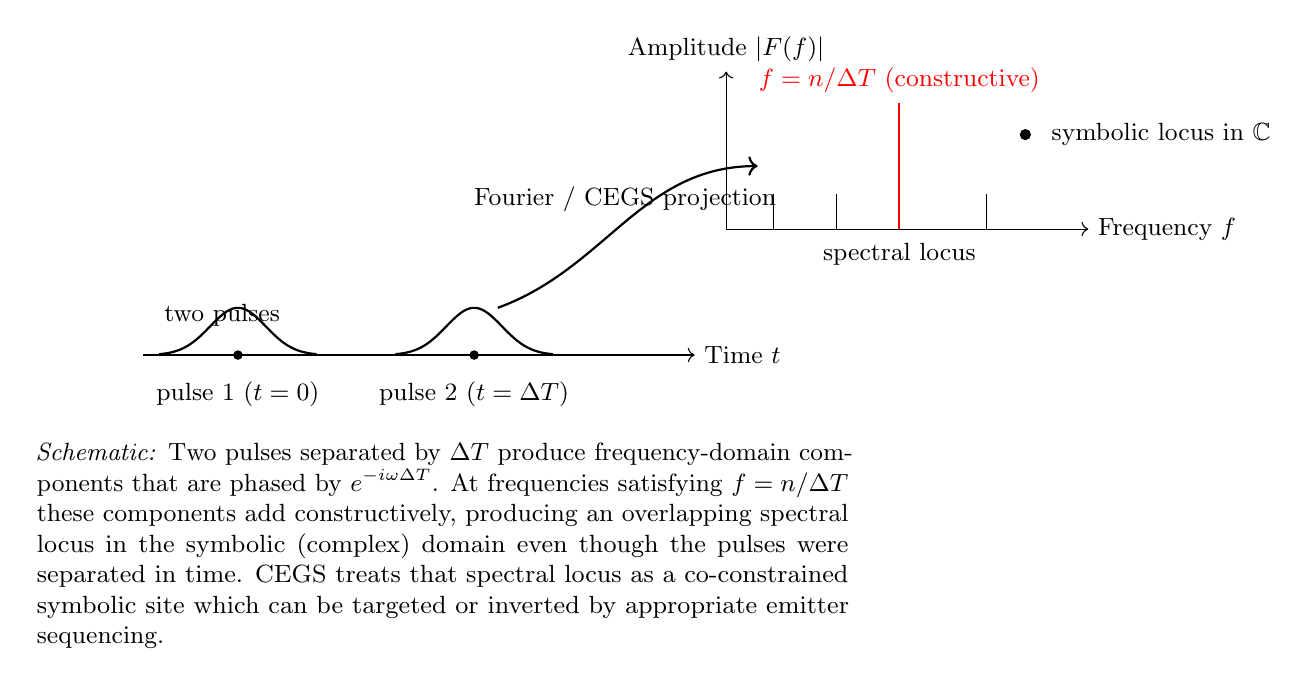
\begin{tikzpicture}[every node/.style={font=\small}, scale=1]
  % Time axis and pulses
  \draw[->] (-0.2,0) -- (6.8,0) node[right] {Time $t$};
  \node at (0.8,0.5) {\small two pulses};
  % pulses
  \draw[fill=black] (1,0) circle (1.5pt) node[below=6pt] {\small pulse 1 $(t=0)$};
  \draw[fill=black] (4,0) circle (1.5pt) node[below=6pt] {\small pulse 2 $(t=\Delta T)$};
  % pulse envelopes
  \draw[thick] plot [domain=0:2,samples=50] (\x, {0.6*exp(-4*(\x-1)^2)});
  \draw[thick] plot [domain=3:5,samples=50] (\x, {0.6*exp(-4*(\x-4)^2)});
  % arrow to frequency domain
  \draw[->, thick] (4.3,0.6) to[out=20,in=180] node[midway,above] {\small Fourier / CEGS projection} (7.6,2.4);

  % Frequency axis and highlighted spectral line
  \begin{scope}[shift={(7.2,1.6)}]
    \draw[->] (0,0) -- (4.6,0) node[right] {Frequency $f$};
    \draw[->] (0,0) -- (0,2.0) node[above] {Amplitude $|F(f)|$};
    % spectral lines (sample)
    \foreach \x in {0.6,1.4,2.2,3.3}{
      \draw[very thin] (\x,0) -- (\x,0.45);
    }
    % highlighted constructive spectral line at f = n / DeltaT
    \draw[thick,red] (2.2,0) -- (2.2,1.6) node[above] {\small $f = n/\Delta T$ (constructive)};
    % label
    \node[below] at (2.2,-0.06) {\small spectral locus};
    % small dot in complex plane to represent symbolic overlap
    \draw[fill=black] (3.8,1.2) circle (1.8pt) node[right=6pt] {\small symbolic locus in $\mathbb{C}$};
  \end{scope}

  % caption-like explanatory text
  \node[below,align=left] at (3.6,-1.0) {\parbox{0.85\textwidth}{\small\textit{Schematic:} Two pulses separated by $\Delta T$ produce frequency-domain components that are phased by $e^{-i\omega\Delta T}$. At frequencies satisfying $f=n/\Delta T$ these components add constructively, producing an overlapping spectral locus in the symbolic (complex) domain even though the pulses were separated in time. CEGS treats that spectral locus as a co-constrained symbolic site which can be targeted or inverted by appropriate emitter sequencing.}};
\end{tikzpicture}
\end{center}

\section*{Conclusion}

We have presented a concise demonstration of how the Calculus of Element-Generated Sets (CEGS)
can be used to encode three-dimensional wavefronts as families of complex-valued function carriers,
how symbolic constraint operations reorganise those families, and how this viewpoint naturally
recasts inverse excitation problems as constraint-inversion tasks. The worked examples show two
roles for CEGS in practice:

\begin{itemize}[leftmargin=*,itemsep=4pt]
  \item As a \emph{conceptual unifier}: CEGS supplies a single symbolic language for divergence,
        functional identities, and constraint closure across mathematics, physics, and symbolic
        computation.
  \item As an \emph{engineering tool}: by lifting metric comparability until constraints are applied,
        CEGS enables reversible encodings and inverse-control formulations that may be more robust
        than purely geometric approaches—especially in situations that exhibit nonlocal or temporal
        coupling (for example, the temporal phase-coupling example above).
\end{itemize}

The practical recipes and worked examples demonstrate how to move from symbolic
specification to implementable emitter signals using classical kernels, discretisation,
and Tikhonov-style inversion, together with adjoint or time-reversal refinements.
Crucially, we highlighted cases where CEGS truly adds value: (i) phase-conjugate or
mirror-symmetric scenarios, (ii) curvature- or surface-coupled wave regimes (plasmonics,
electron–photon coupling), and (iii) temporal-phase coupling where temporally separated
events co-locate in the symbolic domain.



CEGS therefore stands as both a mathematical development and a practical toolkit: a way to
think about divergence, identity, and control symbolically while maintaining a clear line
to actionable engineering formulations. We close with an invitation: test the symbolic inversion
on modest experimental setups (acoustic/microwave) first, where the timings, wavelengths,
and measurement hardware are straightforward, and then scale to higher-frequency or
electron–photon coupling contexts where the deeper novelty of CEGS can be explored.

\vspace{12pt}
\section*{Dissemination and Collaboration Outlook}

The present work establishes the theoretical foundations of the Calculus of Element Generated Sets (CEGS) and demonstrates how geometric wavefronts in $\mathbb{R}^3$ may be encoded and transformed within a complex functional domain. The resulting formulation enables symbolic constraint operations, orthogonality lifting, and reversible mappings between spatial and functional representations — a framework that unifies geometric, algebraic, and wave-propagation viewpoints.

\paragraph{Accessibility and Reproducibility.}
All derivations, figures, and code fragments are openly provided through the Zenodo DOI and corresponding GitHub repository. This ensures complete reproducibility of symbolic constructions and invites further analytical or numerical extension by the community. No experimental facility is required to reproduce the conceptual mappings or to generate the visual demonstrations; all examples can be rendered directly within the included \LaTeX/TikZ environment or translated into computational notebooks.

\paragraph{Collaborative Invitation.}
Researchers active in fields such as wavefield synthesis, symbolic or algebraic geometry, plasmonic field design, or quantum-state modelling are invited to engage with the project through open discussion channels (GitHub or scholarly correspondence). The current exposition is meant as a transparent starting point for collaborative refinement and eventual physical realisation of the proposed constraint-based control principles.

\paragraph{Future Directions.}
Ongoing work aims to: 
(1) extend the symbolic formalism toward nonlocal emitter interference and inverse excitation; 
(2) investigate CEGS-guided numerical kernels for structured field generation; and 
(3) explore the role of constraint geometry in emergent pattern control within optical, acoustic, or electronic media. 
The theoretical accessibility of the framework makes it particularly suited for cross-disciplinary collaboration, where mathematical consistency precedes empirical implementation.

\paragraph{Closing Note.}
By situating CEGS within an openly accessible and symbolic context, this work positions itself not as a finished model but as a generative framework — a map of relations through which other researchers can navigate, test, and extend. 
Dissemination through Zenodo and GitHub, combined with open academic discussion platforms, ensures that constructive engagement remains possible even outside traditional institutional settings.

\vspace{12pt}
\section*{Acknowledgements}

The author gratefully acknowledges the open scientific infrastructure that enables independent theoretical research, particularly the repositories and archival services provided by \textsc{Zenodo} and \textsc{GitHub}. 
Special thanks are extended to the broader open-source and academic communities whose transparent exchange of methods and ideas make such symbolic frameworks possible.

No institutional funding or laboratory resources were employed in this work; all research was conducted independently. 
The project is dedicated to the ideal that mathematical and conceptual innovation should remain freely accessible, reproducible, and extendable by anyone interested in advancing the dialogue between mathematics, physics, and symbolic computation.


\end{document}